\documentclass{beamer}

\usepackage[utf8x]{inputenc} 
\usepackage[slovene,english]{babel}
\usepackage{amssymb}
\usepackage{amsmath}
\usepackage{amsthm}
\usepackage{svg}
\usepackage{ulem}
\usepackage{graphicx}

\usetheme{Madrid}

\setbeamercovered{transparent=25} % pause environment is transparent

% command semitransp to make text semitransparent (actually mixes text with background color to make it appear semitransparent)
\newcommand{\semitransp}[2][25]{\color{fg!#1}#2\color{fg}}

\title{Digitalna topologija na grafih}
\subtitle{Predstavitev diplomskega dela}
\author{Jakob Drusany}
\institute[UL FRI, UL FMF]{Fakulteta za računalništvo in informatiko\\Fakulteta za matematiko in fiziko\\Univerza v Ljubljani}
\date{\selectlanguage{slovene}\today}

\graphicspath{ {../slike/} }


\begin{document}

\begin{frame}
    \titlepage
    {\centering \small Mentor: prof. dr. Petar Pavešić\par}
\end{frame}

% \begin{frame}
% \frametitle{Table of Contents}
% \tableofcontents
% \end{frame}

% Automatically add a table of contents slide at the beginning of each section
% do i need this?
% \AtBeginSection[]
% {
%   \begin{frame}
%     \frametitle{Table of Contents}
%     \tableofcontents[currentsection]
%   \end{frame}
% }

\section{Uvod}
\subsection{Motivacija}
\begin{frame}[t]
    \frametitle{Motivacija}
    Zakaj hočemo topologije na slikah?
\end{frame}
\subsection{Teoretične osnove}

% \begin{frame}[t]
% \frametitle{Teoretične osnove}
% \begin{block}{Definicija}
%     \alert{Topologija} (ali topološka struktura) na množici $X$ je družina $\mathcal{T}$ podmnožic
%     $X$, ki zadošča naslednjim zahtevam:
%     \begin{itemize}
%         \item[(1)] prazna množica in $X$ sta elementa $\mathcal{T}$;
%         \item[(2)] unija poljubne poddružine $\mathcal{T}$ je element $\mathcal{T}$;
%         \item[(3)] presek poljubne končne poddružine $\mathcal{T}$ je element $\mathcal{T}$.
%     \end{itemize}
% \end{block}
% \vspace{.25cm}
% \pause
% Elemente $\mathcal{T}$ imenujemo \alert{odprte množice} v $X$. \alert{Topološki prostor}
% ($X$, $\mathcal{T}$) je množica $X$, opremljena s topologijo $\mathcal{T}$ \\ \vspace{.25cm}
% \alert{Okolica} točke $x \in X$ je vsaka podmnožica $V \subseteq X$, ki vsebuje
% odprto množico $U$, ki vsebuje $x$.
% \end{frame}

% \begin{frame}[t]
% \frametitle{Teoretične osnove}
% \begin{block}{Definicija}
%     \alert{Topologija Aleksandrova} na množici $X$ je družina $\mathcal{T}$ podmnožic
%     $X$, ki zadošča naslednjim zahtevam:
%     \begin{itemize}
%         \item[(1)] prazna množica in $X$ sta elementa $\mathcal{T}$;
%         \item[(2)] unija poljubne poddružine $\mathcal{T}$ je element $\mathcal{T}$;
%         \item[(3)] presek poljubne \sout{končne} poddružine $\mathcal{T}$ je element $\mathcal{T}$.
%     \end{itemize}
% \end{block}
% \pause
% \vspace{.25cm}
% Presek vseh odprtih množic, ki vsebujejo točko $x$ je \alert{najmanjša odprta okolica} točke $x$, ki jo označimo z $U_x$.
% \end{frame}

% \begin{frame}[t]
%     \frametitle{Teoretične osnove}
%     \begin{block}{Definicija}
%         \alert{Simplicialni kompleks} $K$ je sestavljen iz množice $V_K$ in družine $S_K$ podmnožic množice $V_K$, ki zadošča naslednjim pogojem:
%         \begin{itemize}
%             \item[(1)] Vsaka podmnožica $V_K$ moči 1 je element $S_K$.
%             \item[(2)] Vsaka neprazna podmnožica $S_K$ je element $S_K$.
%         \end{itemize}
%     \end{block}
%     \pause
%     \vspace{.25cm}
%     Elemente $V_K$ imenujemo \alert{vozlišča}, elemente $S_K$ pa \alert{simpleksi}.
% \end{frame}

% \section{Končne topologije, delne urejenosti in celični kompleksi}
% \begin{frame}[t] % top align
%     \frametitle{TODO}
%     \vspace{-8mm}
%     % NO TRANSPARENCY
%     \[
%         \text{Delna urejenost}
%         \quad
%         \raisebox{-3pt}{\scalebox{2}{$\substack{\longleftarrow\\[-1em] \longrightarrow }$}}
%         \quad
%         \text{Končna topologija}
%         \quad
%         \raisebox{-3pt}{\scalebox{2}{$\substack{\longleftarrow\\[-1em] \longrightarrow }$}}
%         \quad
%         \text{Celični kompleks}
%     \]
%     \vspace{1cm}
%     NO TRANSPARENCY
% \end{frame}

% \begin{frame}[t] % top align
%     \frametitle{TODO}
%     \vspace{-8mm}
%     % FIRST LEFT 
%     \[
%         \text{Delna urejenost}
%         \quad
%         \raisebox{-3pt}{\scalebox{2}{$\substack{\longleftarrow\\[-1em] \semitransp{\longrightarrow} }$}}
%         \quad
%         \text{Končna topologija}
%         \quad
%         \semitransp{
%             \raisebox{-3pt}{\scalebox{2}{$\substack{\longleftarrow\\[-1em] \longrightarrow }$}}
%             \quad
%             \text{Celični kompleks}
%         }
%     \]
%     \vspace{1cm}
%     FIRST LEFT 
% \end{frame}
% \begin{frame}[t] % top align
%     \frametitle{TODO}
%     \vspace{-8mm}
%     % FIRST RIGHT 
%     \[
%         \text{Delna urejenost}
%         \quad
%         \raisebox{-3pt}{\scalebox{2}{$\substack{\semitransp{\longleftarrow}\\[-1em] \longrightarrow }$}}
%         \quad
%         \text{Končna topologija}
%         \quad
%         \semitransp{
%             \raisebox{-3pt}{\scalebox{2}{$\substack{\longleftarrow\\[-1em] \longrightarrow }$}}
%             \quad
%             \text{Celični kompleks}
%         }
%     \]
%     \vspace{1cm}
%     FIRST RIGHT 
% \end{frame}
% \begin{frame}[t] % top align
%     \frametitle{TODO}
%     \vspace{-8mm}
%     % SECOND LEFT 
%     \[
%         \semitransp{
%             \text{Delna urejenost}
%             \quad
%             \raisebox{-3pt}{\scalebox{2}{$\substack{\longleftarrow\\[-1em] \longrightarrow }$}}
%             \quad
%         }
%         \text{Končna topologija}
%         \quad
%         \raisebox{-3pt}{\scalebox{2}{$\substack{\longleftarrow\\[-1em] \semitransp{\longrightarrow} }$}}
%         \quad
%         \text{Celični kompleks}
%     \]
%     \vspace{1cm}
%     SECOND LEFT 
% \end{frame}
% \begin{frame}[t] % top align
%     \frametitle{TODO}
%     \vspace{-8mm}
%     % SECOND RIGHT 
%     \[
%         \semitransp{
%         \text{Delna urejenost}
%         \quad
%         \raisebox{-3pt}{\scalebox{2}{$\substack{\longleftarrow\\[-1em] \longrightarrow }$}}
%         \quad
%         }
%         \text{Končna topologija}
%         \quad
%         \raisebox{-3pt}{\scalebox{2}{$\substack{\semitransp{\longleftarrow}\\[-1em] \longrightarrow }$}}
%         \quad
%         \text{Celični kompleks}
%     \]
%     \vspace{1cm}
%     SECOND RIGHT 
% \end{frame}
\subsection{Povezava končnih topologij in delnih urejenosti}
\subsection{Simplicialni kompleksi}
\subsection{Povezava topoloških prostorov in simplicialnih kompleksov}

\section{Digitalni prostori}
\subsection{Topologije na grafih}
\begin{frame}[t]
    \frametitle{Topologije na grafih}
    \begin{block}{Definicija}
        Naj bo $G = (V,E)$ graf. Naj bo $\mathcal{T}$ topologija na $V$. $\mathcal{T}$ imenujemo \alert{kompatibilna
        topologija} na $G$, če velja, da je
        $V' \subseteq V$ topološko povezan če in samo če je $G[V']$ grafovsko povezan.
    \end{block}
\end{frame}
\begin{frame}[t]
    \frametitle{Primer kompatibilne topologije}
    \[\mathcal{T}_k = \{\emptyset, \{a\}, \{a, b\}, \{a, b, c\}, \{a, b, d\}, \{a, b, c, d\}\}.\]
    \begin{figure}[h]
        \begin{center}
        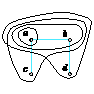
\includegraphics[width=0.3\textwidth]{compatible-topology.pdf}
        \end{center}
    \end{figure}
\end{frame}
\begin{frame}[t]
    \frametitle{Primer topologije na grafu, ki ni kompatibilna}
    \[\mathcal{T}_n = \{\emptyset, \{a\}, \{b\}, \{a, b\}, \{a, c\}, \{a, b, c\}, \{a, b, c, d\}\}.\]
    \begin{figure}[h]
        \begin{center}
        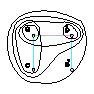
\includegraphics[width=0.3\textwidth]{incompatible-topology.pdf}
        \end{center}
    \end{figure}
\end{frame}
\subsection{Obstoj kompatibilne topologije na grafu}
\subsection{Celični kompleksi}

\begin{frame}[t]
    \frametitle{Kompatibilne topologije na dvodelnih grafih}
    \begin{block}{Izrek}
        Vsak povezan, dvodelen graf $G^b = (V,E)$, ki ima vsaj tri vozlišča, ima natanko
    dve kompatibilni topologiji. To sta $\mathcal{T}_1$ in $\mathcal{T}_2$:
        \[
          \begin{split}
          \mathcal{T}_1:&\quad
          U_x:=\{x\}\ \ \forall x \in V_A, \quad
          U_x:=\{x\}\cup N_x\ \  \forall x \in V_B\\
          \mathcal{T}_2:&\quad
          U_x:=\{x\}\cup N_x\ \  \forall x \in V_A, \quad
          U_x:=\{x\}\ \ \forall x \in V_B\\
        \end{split}
        \]
    \end{block}
\end{frame}
\begin{frame}[t]
    \frametitle{Kompatibilne topologije na dvodelnih grafih}
    \begin{figure}
        \begin{center}
        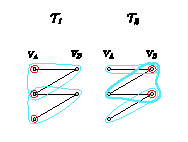
\includegraphics[width=0.5\textwidth]{t1t2_skica.pdf}
        \end{center}
    \end{figure}
    \[
        \begin{split}
        \mathcal{T}_1:&\quad
        U_x:=\{x\}\ \ \forall x \in V_A, \quad
        U_x:=\{x\}\cup N_x\ \  \forall x \in V_B\\
        \mathcal{T}_2:&\quad
        U_x:=\{x\}\cup N_x\ \  \forall x \in V_A, \quad
        U_x:=\{x\}\ \ \forall x \in V_B\\
    \end{split}
    \]
\end{frame}
\begin{frame}[t]
    \frametitle{Kompatibilna topologija na lihem ciklu}
    \begin{block}{Izrek}
    Cikel $C$, ki ima liho število vozlišč $n > 3$, nima kompatibilne topologije.
    \end{block}
    \vspace{1cm}
    $G_v^b := C[\{v\} \cup N_v]$
    \begin{figure}[h]
        \begin{center}
        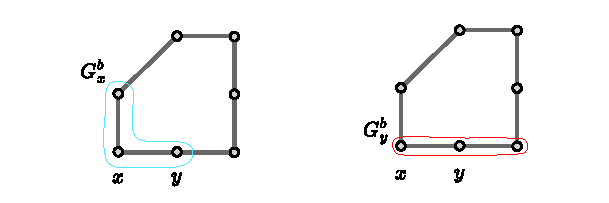
\includegraphics[width=0.8\textwidth]{odd-circle-gb.pdf}
        \end{center}
    \end{figure}
\end{frame}
\begin{frame}[t]
    \frametitle{Kompatibilna topologija na lihem ciklu}
    \begin{figure}[h]
        \begin{center}
        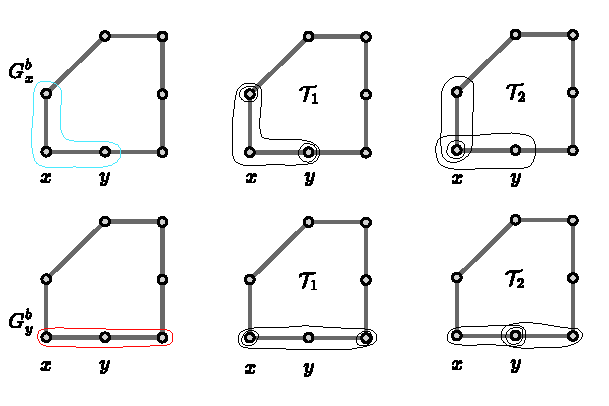
\includegraphics[width=0.8\textwidth]{odd-circle-t1-t2-big.pdf}
        \end{center}
    \end{figure}
\end{frame}
\begin{frame}[t]
    \frametitle{Kompatibilna topologija na lihem ciklu}
    \begin{figure}[h]
        \begin{center}
        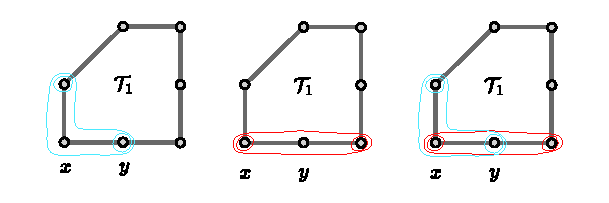
\includegraphics[width=0.8\textwidth]{odd-circle-t1-t2-overlayed.pdf}
        \end{center}
    \end{figure}
    \pause
    Za vsaki dve sosednji točki $x,y \in V(C)$ velja
    \[
    \mathcal{T}|_{V(G_x^b)} \cong \mathcal{T}_1 \iff \mathcal{T}|_{V(G_y^b)} \cong \mathcal{T}_2.
    \]
    sicer bi $U_x = \{x\}$ in $U_y = \{y\}$, kar bi pomenilo, da je množica $\{x, y\}$ nepovezana.
\end{frame}
\begin{frame}[t]
    \frametitle{Obstoj kompatibilne topologije}
    \begin{block}{Izrek}
        Naj bo $G$ graf, v katerem obstaja induciran podgraf, ki je cikel lihe dolžine. Potem
        $G$ nima kompatibilne topologije.
    \end{block}
    \vspace{.5cm}
    \pause
    Zaradi izreka lahko sklepamo, da 8-povezana mreža nima kompatibilne topologije,
    saj v njem obstaja induciran podgraf, ki je cikel lihe dolžine.
    \begin{figure}
        \begin{center}
        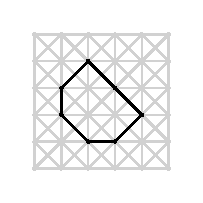
\includegraphics[width=0.35\textwidth]{odd_circle.pdf}
        \end{center}
      \end{figure}
\end{frame}
\end{document}